\section{Materiales y métodos}

\subsection{Datos}

\vspace{0,3cm}

\subsubsection*{Datos del fenotipo}

Para este estudio, se utilizó el fenotipo Demencia frontotemporal, identificado con el término HP:0002145 en Human Phenotype Ontology (HPO). A partir de este término HPO, se han extraído 52 genes asociados al fenotipo. Estos genes se obtuvieron mediante la API Ontology Annotation Network \cite{hpo_api} de HPO, que permite acceder programáticamente a las anotaciones entre términos fenotípicos y genes. A través de esta API, se descargaron los datos en formato JSON, que luego fueron procesados para extraer los nombres de los genes y guardarlos en un archivo TSV.

Estos genes, relacionados con el desarrollo de la demencia frontotemporal y otras patologías neurodegenerativas, representan el conjunto inicial de genes sobre el que se construirá la red de interacciones para el análisis posterior. Cada uno de ellos se identifica mediante su ID único en la base de datos de NCBIGene, lo cual facilita el acceso y la referencia a los datos genéticos específicos.

Para asegurar la reproducibilidad, se utilizó la versión 2.0.4 de HPO  \cite{HPO}, para obtener el término fenotípico y descargar los genes relacionados con el fenotipo de estudio. En la siguiente sección se proporciona una descripción detallada de HPO.
 
\subsubsection*{Human Phenotype Ontology (HPO)}

HPO proporciona una ontología estandarizada que describe anomalías fenotípicas observadas en enfermedades humanas, facilitando la identificación y análisis de genes asociados a diversas características clínicas. Cada término en HPO representa una anomalía específica, como la demencia frontotemporal, y está diseñado para facilitar la caracterización precisa de los fenotipos en el contexto de enfermedades hereditarias. La ontología se desarrolla y actualiza de forma continua utilizando fuentes como la literatura médica, así como bases de datos como Orphanet, DECIPHER y OMIM. Actualmente, HPO contiene más de 18,000 términos y ofrece más de 156,000 anotaciones asociadas a enfermedades hereditarias \cite{HPO}.


\subsubsection*{Datos de interacción}

Los datos de interacción representan conexiones funcionales y físicas entre proteínas, y constituyen la base para construir redes de interacción en el análisis de procesos biológicos. En este estudio, los datos de interacción proteína-proteína (PPI) fueron extraídos de la base de datos STRING mediante su API REST \cite{string_api}, que permite recuperar programáticamente redes de interacción específicas basadas en listas de genes o proteínas de interés.

A través de esta API, se obtuvieron las interacciones entre los genes asociados al fenotipo FTD (HP:0002145) en formato TSV. En este archivo, cada fila representa una interacción entre dos proteínas y contiene las siguientes columnas.

\begin{itemize}
	\item \textbf{protein1:} ID de la primera proteína en la interacción, precedido por el código taxonómico del organismo (por ejemplo, "9606" para proteínas humanas).
	\item \textbf{protein2:} ID de la segunda proteína en la interacción, también con el prefijo de organismo.
	\item \textbf{combined\_score:} Puntuación de confianza combinada para cada interacción proteína-proteína, con valores que oscilan entre 0 y 1000. Esta puntuación refleja la probabilidad de que una interacción sea real, basada en una integración de diversas fuentes de evidencia, como co-ocurrencia filogenética, co-expresión, minería de texto y datos experimentales. Cada tipo de evidencia se evalúa y puntúa individualmente, y luego se combina en el "combined\_score", proporcionando así un indicador global de confiabilidad para cada interacción funcional o física \cite{szklarczyk2023stringdb}.
\end{itemize}

Estos datos obtenidos se utilizarán para construir una red de interacciones entre los genes asociados al fenotipo FTD, permitiendo analizar las relaciones funcionales entre proteínas en este contexto. Esta red servirá como base para el análisis de clustering, facilitando la identificación de módulos de genes potencialmente implicados en funciones biológicas específicas.

Para asegurar la reproducibilidad del análisis, se utilizó la versión 12.0 de STRING, junto con su API REST de STRING para la extracción de interacciones.


\subsubsection*{STRING}
La base de datos STRING (Search Tool for the Retrieval of Interacting Genes/Proteins) es un recurso bioinformático diseñado para recopilar, organizar y analizar redes de interacciones proteína-proteína y asociaciones funcionales en cualquier genoma secuenciado. STRING integra información de diversas fuentes, como minería de texto científico, predicciones computacionales basadas en coexpresión y contexto genómico, y datos experimentales obtenidos de estudios de interacciones proteicas. Además, los usuarios pueden acceder a la base de datos para explorar redes de interacción, realizar análisis de enriquecimiento funcional y generar redes personalizadas para genomas específicos, facilitando así la investigación en biología celular y molecular. Actualmente, STRING cubre 59.309.604 proteínas provenientes de 12.535 organismos.  \cite{szklarczyk2023stringdb}.

\subsection{Software}

Para el análisis funcional y la construcción de redes genéticas en este estudio, se seleccionaron herramientas especializadas que permiten tanto la exploración bioinformática como la visualización de datos complejos. Dado que el objetivo principal es investigar la interacción entre genes y módulos específicos asociados a la demencia frontotemporal, se ha optado por una combinación de paquetes en Python que ofrecen un balance entre precisión analítica y capacidades visuales avanzadas.

\subsection*{Paquetes de Python para el análisis funcional y otras funciones}

\begin{itemize}
	\item \textbf{NumPy (versión 1.26.0)}: Esta librería proporciona soporte para arrays multidimensionales y funciones matemáticas de alto rendimiento. Es fundamental para realizar cálculos numéricos eficientes y operaciones matemáticas en grandes conjuntos de datos \cite{numpy}.
	\item \textbf{Pandas (versión 2.2.3)}: Este paquete proporciona estructuras de datos eficientes y flexibles, como DataFrames, que facilitan el procesamiento y manipulación de datos complejos. En el contexto de este estudio, Pandas permite organizar, filtrar y procesar resultados de enriquecimiento funcional, simplificando el manejo de grandes volúmenes de datos bioinformáticos \cite{pandas}.
	\item \textbf{Stringdb (versión 1.1.0)}: Un paquete que facilita el acceso a la base de datos STRING para recuperar información sobre interacciones proteicas y realizar análisis de enriquecimiento \cite{stringdb}.
	\item \textbf{Requests (versión 2.31.0)}: Requests es una biblioteca para realizar solicitudes HTTP de manera simple y efectiva. En este estudio, se utiliza para conectar con APIs externas como la de STRINGdb, permitiendo la descarga automatizada de datos de redes y enriquecimiento \cite{requests}.
	\item \textbf{GSEAPY (versión 1.0.5)}: GSEAPY permite realizar análisis de enriquecimiento funcional y análisis de vías de manera sencilla, integrando métodos como GSEA y prerank para conjuntos de genes. Es fundamental para identificar procesos biológicos relevantes en los genes analizados \cite{gseapy}.
	\item \textbf{Igraph (versión 0.10.8)}: Una biblioteca para la creación, manipulación y visualización de grafos y redes complejas. Es esencial para representar y analizar redes de interacciones génicas y otros tipos de grafos en el contexto de estudios bioinformáticos \cite{igraph}.
	\item \textbf{NetworkX (versión 3.1)}: Esta librería facilita el análisis y visualización de estructuras de grafos y redes complejas. Se aplica para modelar y visualizar redes de interacciones génicas \cite{networkx}.
	\item \textbf{Matplotlib (versión 3.8.1)}: Matplotlib es una librería de visualización muy versátil que soporta múltiples tipos de gráficos en 2D, lo que resulta útil para representar tendencias y relaciones entre genes en gráficos de líneas, barras, dispersión, y más. Se pondrán en uso extensiones como las de Colors, CM, Axes, Patches. Este paquete se utilizará para visualizar los resultados de enriquecimiento y las interacciones génicas \cite{matplotlib}.
	\item \textbf{Matplotlib-Venn (versión 0.11.9)}: Esta librería permite crear diagramas de Venn con Matplotlib para representar gráficamente las relaciones entre conjuntos de datos \cite{matplotlibvenn}.
	\item \textbf{UpSetPlot (versión 0.8.0)}: UpSetPlot es una herramienta para crear gráficos de tipo UpSet, que permiten visualizar intersecciones entre conjuntos de datos, útil en el análisis de enriquecimiento funcional \cite{upsetplot}.
	\item \textbf{Seaborn (versión 0.12.2)}: Seaborn es una librería de visualización basada en Matplotlib que permite crear gráficos estadísticos atractivos y con estilo. Se utiliza para explorar y visualizar patrones y relaciones en los datos \cite{seaborn}.
	\item \textbf{Plotly (versión 5.18.0)}: Plotly es una biblioteca interactiva para crear gráficos y visualizaciones avanzadas. Se utiliza para representar redes e interacciones complejas de forma dinámica y visualmente atractiva \cite{plotly}.
	\item \textbf{Scienceplots (versión 2.1.1)}: Este paquete extiende Matplotlib proporcionando estilos de gráficos estéticamente optimizados para publicaciones científicas. Con Scienceplots, se puede lograr una presentación visual de alta calidad, ideal para gráficos que requieren una apariencia profesional \cite{scienceplots}.
	\item \textbf{Argparse (versión 1.4.0)}: Argparse es una librería estándar para analizar argumentos en la línea de comandos, facilitando la ejecución flexible de scripts y automatización de tareas \cite{argparse}.
	\item \textbf{Logging (versión 0.5.1.2)}: Logging es un módulo estándar que permite registrar mensajes y eventos durante la ejecución de los scripts, lo que facilita el seguimiento y depuración del proceso de análisis \cite{logging}.
	\item \textbf{Shutil (módulo estándar)}: Permite realizar operaciones con archivos y directorios, como copiar, mover o eliminar, facilitando el manejo del sistema de archivos en los scripts \cite{shutil}.
	\item \textbf{JSON (módulo estándar)}: Este módulo facilita la manipulación y el intercambio de datos en formato JSON, útil para procesar configuraciones y respuestas de APIs \cite{json}.
	\item \textbf{Time (módulo estándar)}: Proporciona funciones para medir el tiempo de ejecución y realizar pausas en los scripts, lo que facilita el control del flujo de trabajo \cite{time}.
	\item \textbf{Re (módulo estándar)}: Este módulo permite realizar operaciones con expresiones regulares, facilitando la búsqueda y manipulación de cadenas de texto \cite{re}.
	\item \textbf{Platform (módulo estándar)}: Proporciona información sobre el sistema operativo y el entorno de ejecución, útil para adaptar el comportamiento de los scripts según el entorno \cite{platform}.
	\item \textbf{Random (módulo estándar)}: Facilita la generación de números aleatorios, útil en procesos de muestreo o simulación \cite{random}.
	\item \textbf{Psutil (versión 5.9.5)}: Permite monitorizar el uso de recursos del sistema, como memoria y CPU, lo cual es útil para optimizar el rendimiento de los scripts \cite{psutil}.
	\item \textbf{YAML (versión 6.0)}: Facilita la lectura y escritura de archivos YAML, útil para manejar configuraciones en un formato legible y estructurado \cite{yaml}.
	\item \textbf{Optuna (versión 3.5.0)}: Una librería para la optimización automática de hiperparámetros en modelos y algoritmos, mejorando el rendimiento del análisis \cite{optuna}.
	\item \textbf{Math (módulo estándar)}: Proporciona funciones matemáticas básicas como logaritmos y raíces cuadradas, necesarias para realizar cálculos en el análisis funcional \cite{math}.
	\item \textbf{Itertools (módulo estándar)}: Proporciona funciones para crear iteradores eficientes, como combinaciones y permutaciones, útiles para el análisis de redes y conjuntos de datos \cite{itertools}.
	\item \textbf{Jinja2 (versión 3.1.3)}: Un motor de plantillas para Python que permite generar contenido dinámico, útil para personalizar informes y representaciones visuales \cite{jinja2}.
	\item \textbf{Kaleido (versión 0.2.1)}: Una herramienta para exportar gráficos de Plotly a formatos estáticos como PNG, PDF y SVG, facilitando la creación de visualizaciones de alta calidad \cite{kaleido}.
	

\end{itemize}


\subsection{Análisis de enriquecimiento de vías biológicas}

El análisis de enriquecimiento permite identificar vías biológicas o pathways que están significativamente representados en una lista de genes de interés, por medio de pruebas estadísticas. Un pathway es un conjunto de genes que trabajan en conjunto para llevar a cabo un proceso biológico específico.\cite{Reimand2019}

En este estudio, se realizó un análisis de enriquecimiento para las agrupaciones de genes derivadas del algoritmo de clustering que ha generado un mejor resultado.

Las herramientas de análisis funcional mapean las listas de genes de interés a terminos biólógicos anotados, como los términos GO y utilizan métodos estadísticos, como el test de Ficher o test hipergeométricos,
para evaluar el enriquecimiento.\cite{10.1093/nar/gkn923} En particular, el test hipergeométrico evalúa si la representación de cada término funcional en el conjunto de genes de interés 
es mayor que la esperada por azar. 


Para la realización de este análisis funcional se ha hecho uso del módulo \textit{enrich} de biblioteca de Python \textit{GSEAPY} que permite la realización de un 
análisis de enriquecimiento de una lista de genes mediante la utilización de la API de Enrich. Esta herramienta evalúa si un conjunto de genes de entrada se superpone significativamente con conjuntos de genes previamente anotados. 
El análisis se ha realiza utilizando la base de datos  GO\_Biological\_Process\_2021, que recopila información sobre procesos biológicos. Sin embargo, la utilización de otras ontologías como 
Gene Ontology (GO), UniProt, Reactome o KEGG podrían  información complementaria sobre diferentes tipos de términos funcionales.

Enrich va a proporcionar varias métricasa a cerca de los resultados del enriquecimiento: p-valor, p-valor ajustado, odds ratio y combined score.
El p-valor, calculado las pruebas estadísticas anteriormente mencionadas evalúa la significancia estadística de la superposición entre los genes de interés y los anotados en los términos. El p-valor ajustado
utilizando el método de Benjamini-Hochberg para controlar la tasa de falsos positivo. La métrica de odds ratio mide la proporción entre los genes superpuestos observados y los esperados bajo una distribución aleatoria.
Finalmente, combined score combina el p-value y el odds ratio en una métrica única. \cite{maayanlab_enrichr_help}

Finalmente, se aplicaron filtros para seleccionar únicamente los términos funcionales más relevantes en los resultados obtenidos. Estos filtros han sido el p-valor ajustado a  0.005,
combined score a  2000 y el porcentaje de overlap que se ha definico como  el número de genes de la lista de interés que se suporponen con los genes anotados del término entre el total de genes anotados en el término a 0.1.




\subsection{Clustering}

Al aplicar algoritmos de clustering, nuestro objetivo es descubrir comunidades funcionales dentro de la red de genes asociada a la demencia frontotemporal. Estas comunidades, módulos, o \textit{clusters} funcionales pueden representar procesos biológicos específicos, vías celulares, o mecanismos asociados al fenotipo FTD. Encontrar estos clusters podría revelar posibles dianas terapéuticas o grupos de biomarcadores dentro del conjunto de genes, lo cual podría abrir las puertas a nuevos tratamientos para los pacientes de FTD.

\subsubsection{Red}

En la red de interacción proteína-proteína (PPI) obtenida mediante la API de STRINGdb, cada nodo representa un gen y cada arista representa una interacción entre genes, ponderada por un puntaje de confianza otorgado por STRINGdb \cite{szklarczyk2023stringdb}. Para enfocarnos en interacciones más sólidas y confiables, se aplicó un umbral mínimo de confianza en las aristas, lo que permitió refinar la red y mejorar la relevancia de los clústeres detectados. 

% (\textbf{NOTA:} Se debe ahondar en esto si al final se hace: ¿Por qué ese umbral? ¿Y si fueran otros umbrales?).

\subsubsection{Algoritmos}
\label{sec:algoritmos}

A continuación, se detallan los tres algoritmos de clustering, proporcionados por la librería \textit{iGraph}, elegidos para este estudio, los cuales pretenden cubrir diferentes enfoques teóricos en la detección de comunidades funcionales \cite{igraph}.  

\textit{Walktrap}: Algoritmo de clustering jerárquico aglomerativo que detecta comunidades basándose en la probabilidad de que recorridos aleatorios dentro de la red permanezcan dentro de clústeres cohesivos \cite{pons2005walktrap}. El algoritmo aplica recorridos aleatorios para capturar la proximidad de los nodos, asumiendo que los nodos que pertenecen a la misma comunidad tienen mayores probabilidades de estar conectados mediante recorridos cortos. Comienza con cada nodo como su propio clúster, fusionando sucesivamente los clústeres cercanos hasta alcanzar una partición óptima. Se ajustó la longitud de los pasos (\textit{steps}).

\textit{Algoritmo de Leiden}: Se basa en optimizar el Constant Potts Model (CPM) de la red \cite{traag2019leiden,constantplottsmodel}. Esta función, mostrada en la Ecuación \ref{eq:cpm}, evalúa la calidad de una partición en comunidades considerando un balance entre la densidad interna de cada clúster y el parámetro de resolución \(\gamma\), que controla el tamaño preferido de las comunidades finales. El término \(n_c\) se refiere al número de nodos, mientras que \(e_c\) es el número de aristas internas, ambos referidos a la comunidad \(c\).

\begin{equation}
	\label{eq:cpm}
	\mathcal{H} = \sum_{c} \left[ e_c - \gamma \left( \frac{n_c (n_c - 1)}{2} \right) \right]
\end{equation}

\noindent Se ajustó el parámetro \(\gamma\), así como el número de iteraciones del algoritmo, permitiendo que el Leiden refinara iterativamente la partición. El resto de parámetros se fijaron a su valor por defecto. 

% (\textbf{NOTA:} Hay un parámetro intersante, \textit{initial\_membership} el cual son nodos 'semilla' que se pasan como argumento, y el algoritmo intenta mejorar las comunidades alrededor de estos nodos. Podríamos usar genes del análisis funcional como semilla y ver qué pasa.)

\textit{Algoritmo de Louvain}: Este algoritmo optimiza la modularidad de la red, una métrica que mide la calidad de una partición en comunidades al comparar la densidad de conexiones internas con la densidad esperada si las conexiones fueran aleatorias \cite{Blondel2008Louvain}. La modularidad \( Q \), definida en la Ecuación \ref{eq:modularity}, es un valor escalar entre \(-1\) y \(1\) que representa la diferencia entre la densidad de aristas dentro de las comunidades y la densidad de aristas esperada. El algoritmo Louvain maximiza esta modularidad en dos fases, cuyo resultado es la formación una nueva red sobre la cual se repite el proceso hasta que la modularidad no mejore más. En redes ponderadas, los autores del algoritmo expresaron la modularidad a optimizar como:

\begin{equation}
	\label{eq:modularity}
	Q = \frac{1}{2m} \sum_{i,j} \left[ A_{ij} - \frac{k_i k_j}{2m} \right] \delta(c_i, c_j),
\end{equation}

\noindent donde \( A_{ij} \) es el peso de la arista entre los nodos \( i \) y \( j \), \( k_i \) y \( k_j \) son las sumas de los pesos de las aristas conectadas a los nodos \( i \) y \( j \), \( c_i \) y \( c_j \) representan las comunidades a las que pertenecen los nodos \( i \) y \( j \), y \( \delta(c_i, c_j) \) es una función delta de Kronecker que es 1 si \( c_i = c_j \) y 0 en caso contrario. El término \( m \) es la suma total de los pesos de las aristas en la red.

\noindent Se ajustó el parámetro de resolución, que controla el tamaño final de las comunidades. El resto de parámetros se dejaron con sus valores por defecto.

\subsubsection{Medidas de Rendimiento}
\label{sec:metricas}

\subsubsection{Optimización}

Como se explicó en la Sección \ref{sec:algoritmos}, Louvain y Leiden son algoritmos de clustering con múltiples parámetros configurables. Ajustar adecuadamente estos parámetros es crucial para mejorar tanto la interpretación biológica de la red como la detección de comunidades. Este proceso, conocido como ajuste de hiperparámetros, busca optimizar el rendimiento del algoritmo según diversas métricas. En este apartado, se detalla el procedimiento empleado para ajustar el parámetro de resolución (\(\gamma\)) en Leiden y Louvain, con el objetivo de maximizar las métricas descritas en la Sección \ref{sec:metricas}.

La estadística bayesiana es un enfoque probabilístico que utiliza el teorema de Bayes para actualizar las creencias sobre un modelo a medida que se incorporan nuevos datos. El ajuste bayesiano de hiperparámetros (BHO) aplica este enfoque para optimizar los parámetros de un modelo, construyendo y actualizando iterativamente un modelo probabilístico de la función objetivo en función de los hiperparámetros. Este modelo probabilístico sugiere los hiperparámetros a probar en cada iteración, permitiendo enfocar eficientemente la búsqueda en las regiones más prometedoras del espacio de hiperparámetros.

Existen diversos algoritmos basados en BHO, cada uno caracterizado por el modelo probabilístico que construye. En este proyecto, hemos optado por el Tree-structured Parzen Estimator (TPE). En el TPE, consideramos que \( y \) es el valor obtenido al evaluar la función objetivo utilizando un conjunto de hiperparámetros \( \theta \). Definimos un umbral \( y^* \) que nos permite dividir nuestros datos en dos conjuntos: los hiperparámetros que resultan en un rendimiento mejor que \( y^* \) y los que resultan en un rendimiento peor. Es decir:

\begin{equation}
	\begin{aligned}
		\mathcal{C}_1 = \left\{ \theta^{(i)} \mid y^{(i)} \leq y^* \right\} \\
		\mathcal{C}_2 = \left\{ \theta^{(i)} \mid y^{(i)} > y^* \right\}
	\end{aligned}
\end{equation}

Utilizando estimación de densidad por kernel (KDE), en este caso, el método de ventana deslizante de Parzen-Rosenblatt -ver detalles en Sección \ref{sec:anexo_a}- estimamos las distribuciones de probabilidad para estos dos conjuntos:

\begin{equation}
	\begin{aligned}
		l(\theta) &= p(\theta \mid \theta \in \mathcal{C}_1) \\
		g(\theta) &= p(\theta \mid \theta \in \mathcal{C}_2)
	\end{aligned}
\end{equation}

El objetivo es seleccionar nuevos hiperparámetros \( \theta \) que maximicen el Expected Improvement (EI), que es proporcional al cociente de estas dos densidades:

\begin{equation}
	\mathrm{EI}(\theta) \propto \frac{l(\theta)}{g(\theta)}
\end{equation}

Al maximizar \( \mathrm{EI}(\theta) \), favorecemos los hiperparámetros que son más probables en el conjunto de buen rendimiento \( \mathcal{C}_1 \) y menos probables en el conjunto de peor rendimiento \( \mathcal{C}_2 \). Este proceso se repite iterativamente; en cada iteración, los nuevos datos de rendimiento actualizan \( l(\theta) \) y \( g(\theta) \), permitiendo explorar eficientemente el espacio de hiperparámetros.

Para Louvain y Leiden, se han ejecutado, respectivamente, \(150\) iteraciones, explorando resoluciones entre \(0.1\) y \(2.0\) que maximicen tanto el coeficiente Q como el puntuaje FES, descritos en la Sección \ref{sec:metricas}. Los datos se han almacenado en una base de datos SQLite, lo que permite extraer informes tabulados y reanudar el ajuste desde el punto de guardado si se desea, facilitando la gestión y continuidad del proceso.


Como se comentó anteriormente, el principal objetivo del clustering en nuestra red PPI es determinar las comunidades funcionales subyacentes con la finalidad de identificar rutas metabólicas compatibles con la elaboración de dianas o biomarcadores para el tratamiento de la FTD. Por esto, no se debe perder la interpretabilidad biológica de la red, a la vez que se intenta maximizar la calidad del clustering aplicado. Dadas estas condiciones, se propone una optimización multiobjetivo, repartiendo las tareas de significancia biológica y calidad del clustering entre las siguientes métricas:

\begin{itemize}
	\item \textit{Modularidad (Q)}. Destinada a la evaluación de la calidad del clustering aplicado. Valores altos indican una conectividad interna densa dentro de los clústeres y conexiones dispersas entre ellos. La alta modularidad sugiere comunidades bien definidas.
	
	\item \textit{Puntaje de Enriquecimiento Funcional}: Para cada clúster, se realizó un análisis de enriquecimiento funcional mediante STRINGdb. Este puntaje refleja la significancia estadística de pathways, términos de la Ontología de Genes u otras anotaciones funcionales enriquecidas dentro de los clústeres. Un puntaje alto indica mayor relevancia biológica, ya que los clústeres enriquecidos en términos específicos probablemente representan procesos biológicos significativos.
\end{itemize}


\subsubsection*{Optimización}
Se generaron varias configuraciones de modelos al ajustar sistemáticamente los parámetros de los algoritmos y evaluamos cada configuración en base a modularidad y puntaje de enriquecimiento funcional. Al trazar estos puntajes en un frente de Pareto, identificamos las configuraciones que representan el mejor equilibrio entre coherencia estructural (modularidad) y relevancia biológica (enriquecimiento funcional) \cite{goodarzi2014PARETOFRONT1,jahan2013multiPARETOFRONT2,costa2015paretoPARETOFRONT3}. Las configuraciones a lo largo de esta frontera representan soluciones Pareto-eficientes de clustering, donde mejorar una métrica no compromete significativamente la otra, permitiendo explorar soluciones con un balance diferente de las métricas de rendimiento elegidas.

% \textbf{NOTA:} Podríamos aplicar algún algoritmo interesante de ajuste de los hiperparámetros, yo (Mario) tengo experiencia aplicando Tree-structured Parzen Estimator y otros algoritmos de ajuste Bayesiano en Python.

\begin{figure}[h]
	\centering
	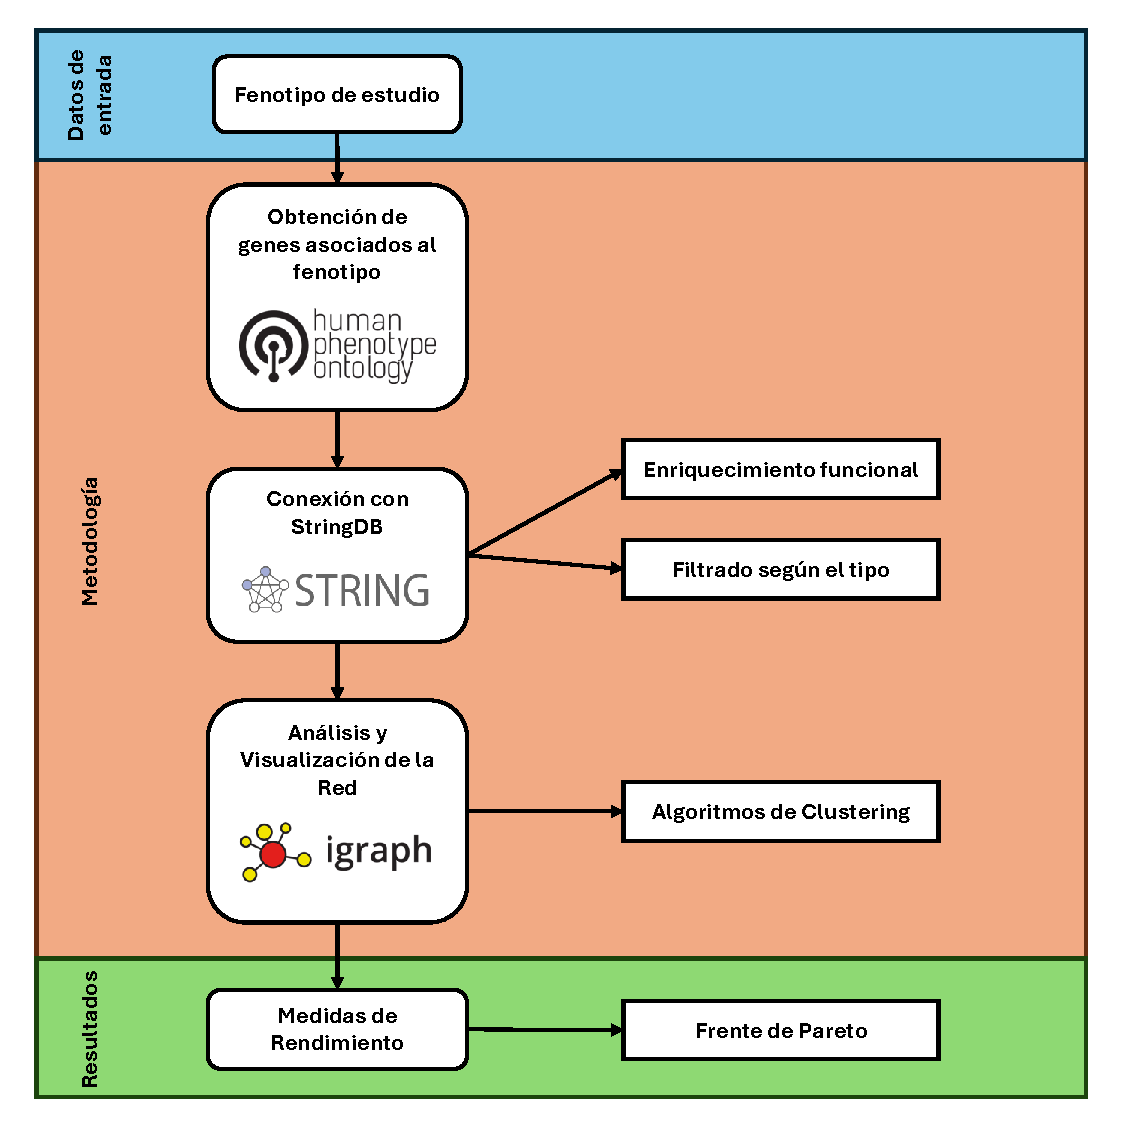
\includegraphics[width=1\linewidth]{figures/methods/Flujo_de_trabajo.pdf}
	\caption{Flujo de trabajo que se seguirá durante el desarrollo del proyecto, partiendo del fenotipo como dato de entrada, metodología y análisis de resultados.}
	\label{fig:flujo_trabajo}
\end{figure}
